\documentclass[sn-basic]{sn-jnl}

\usepackage[T1]{fontenc}
\usepackage[utf8]{inputenc}
\usepackage{lmodern}
\usepackage{amsmath,amssymb,mathtools}
\usepackage{graphicx,booktabs}
\usepackage{siunitx}
\usepackage{microtype}
\usepackage[numbers]{natbib}

\setlength{\emergencystretch}{3em}
\sloppy

\graphicspath{{figures/}}

\jyear{2025}
\title[Symbolic Wavefunctions and Entropic Fractals]
{Symbolic Wavefunctions and Entropic Fractals: A Structural--Analogical Heuristic for Socio--Symbolic Dynamics}

\author*[1]{\fnm{Demetrios} \sur{Agourakis}}\email{demetrios@agourakis.med.br}
\affil[1]{\orgname{Faculdade São Leopoldo Mandic}, \orgaddress{\city{Campinas}, \country{Brazil}}}
\affil[ ]{\orgname{PUC-SP (MSc in Biomaterials and Regenerative Medicine)}, \orgaddress{\city{São Paulo}, \country{Brazil}}}
\thanks{ORCID: 0000-0002-8596-5097}

\keywords{philosophy of science; structural analogy; complex systems; fractals; entropy; quantum-like models; socio-symbolic dynamics; methodology}

\abstract{
We advance a formal--analogical framework that conceives social organization as an \emph{entropically driven fractal dynamics}. A symbolic Schr\"odinger--like representation uses a normative potential \(V(x)\) for cultural constraints and a symbolic mass \(m_s\) for identity inertia; the symbolic wavefunction \(\psi_s(x,t)\) induces densities \(|\psi_s|^2\) on a socio--symbolic space. Crucially, the quantum machinery is treated as a \emph{structural analogy}---not a physical mechanism. We articulate falsifiable signatures (scaling exponents \citep{West1997,Bettencourt2007}, cascade statistics \citep{Bak1987,ClausetShaliziNewman2009,StumpfPorter2012,Alstott2014}, order--effects \citep{BusemeyerBruza2012,HavenKhrennikov2013}), outline estimation of \(V(x)\) and \(m_s\), and present a concise SWOW--style proof--of--concept. The contribution is a disciplined mapping that preserves explanatory payoff for social emergence and cognitive--affective coupling while avoiding category mistakes \citep{Hesse1966,Cartwright1983,FriggHartmannSEP}.}

\begin{document}
\maketitle

\section{Introduction}\label{sec:intro}
We propose a structural--analogical formalism to model socio--symbolic dynamics via a symbolic wavefunction \(\psi_s(x,t)\) evolving under a normative potential \(V(x)\) and a symbolic mass \(m_s\).
The approach converses with small--world \citep{WattsStrogatz1998} and scale--free organization \citep{BarabasiAlbert1999}, self--organized criticality \citep{Bak1987}, and scaling regularities in complex systems \citep{West1997,Bettencourt2007}, while aligning with philosophical accounts of models and analogies \citep{Hesse1966,Cartwright1983,FriggHartmannSEP}.
Our goal is to maintain falsifiability and operational clarity without physical reduction.

\section{Method and Epistemic Status}\label{sec:method}
We take the symbolic evolution
\begin{equation}
i\hbar\,\partial_t \psi_s \;=\; \Big[-\frac{\hbar^2}{2m_s}\nabla^2 + V(x)\Big]\psi_s,\qquad x\in X\subset\mathbb{R}^d,
\end{equation}
as an \emph{analogy of structure} \citep{Hesse1966}.
Here, \(V(x)\) encodes normative--cultural constraints; \(m_s\) encodes identity inertia; \(|\psi_s|^2\) is a density of manifestation.
Interference patterns correspond to non--additivity/order effects \citep{BusemeyerBruza2012,HavenKhrennikov2013}; tunnelling analogs capture barrier crossing under strong constraints.
No ontological commitment to quantum substrates is made.

\subsection{Mapping (QM $\to$ Social)}
\begin{table}[t]
\centering
\small
\resizebox{\linewidth}{!}{%
\begin{tabular}{ll}
\toprule
\textbf{QM element} & \textbf{Social counterpart}\\
\midrule
$\psi(x,t)$ & $\psi_s(x,t)$: socio--symbolic amplitude\\
$|\psi|^2$ & $|\psi_s|^2$: density of manifestation\\
$-\frac{\hbar^2}{2m}\nabla^2 + V(x)$ & $-\frac{\hbar^2}{2m_s}\nabla^2 + V(x)$\\
$\nabla^2$ & diffusion/transition propensity in symbolic space\\
$m$ & $m_s$: identity inertia/rigidity\\
$V(x)$ & normative--cultural field/cost of deviation\\
Interference & non--additive discursive coupling/order effects\\
Tunnelling & improbable transitions across norms\\
\bottomrule
\end{tabular}%
}
\caption{Structural mapping from quantum formalism to socio--symbolic dynamics.}
\label{tab:mapping}
\end{table}

\section{Testable Signatures}\label{sec:signatures}
\begin{center}
\begin{tabular}{lll}
\toprule
Variable & Signature & Metric/Operationalization\\
\midrule
\(m_s\) & slower trajectories; rigidity & path entropy; embedding drift; Hurst exponent\\
\(V(x)\) & alignment; confinement; tunnelling & GP/regression for \(V\); change-points; transition hazard\\
\(|\psi_s|^2\) & dense pockets; non-additivity & cluster overlap; Jensen--Shannon divergence; order tests\\
\(\nabla^2\) & smoothing/propagation & Laplacian; total variation; diffusion coefficients\\
SOC cascades & heavy-tailed sizes & power-law inference \citep{ClausetShaliziNewman2009,StumpfPorter2012,Alstott2014}\\
Metastability & dwell + jumps & dwell-time; CUSUM/PELT\\
Interference & order-dependence & quantum-like decision paradigms \citep{BusemeyerBruza2012,HavenKhrennikov2013}\\
\bottomrule
\end{tabular}
\end{center}

\section{Estimation Blueprint}\label{sec:estimation}
Construct \(X\) using language embeddings/behavioral features; estimate \(V(x)\) with penalized regression or Gaussian processes; infer \(m_s\) from identity persistence and dwell times; validate with diffusion baselines and synthetic recovery.

\section{Proof-of-Concept (SWOW-style)}\label{sec:poc}
We illustrate rank--frequency structure and salient cue\(\to\)response links using a small SWOW-style subset, as in large-scale word association studies \citep{WattsStrogatz1998,BarabasiAlbert1999}.

\section{Objections and Limits}\label{sec:limits}
No physical reduction is claimed; the analogy is structural \citep{Hesse1966,Cartwright1983}.
Identifiability of \(V(x)\) and \(m_s\) requires longitudinal data; ethical notes include transparency on assistive AI and dataset licenses.

\section{Conclusion}\label{sec:conclusion}
A disciplined mapping from quantum formalism to socio--symbolic dynamics with falsifiable signatures \citep{ClausetShaliziNewman2009,StumpfPorter2012,Alstott2014} and a practicable estimation path from data to explanation.

\begin{figure}[t]
\centering
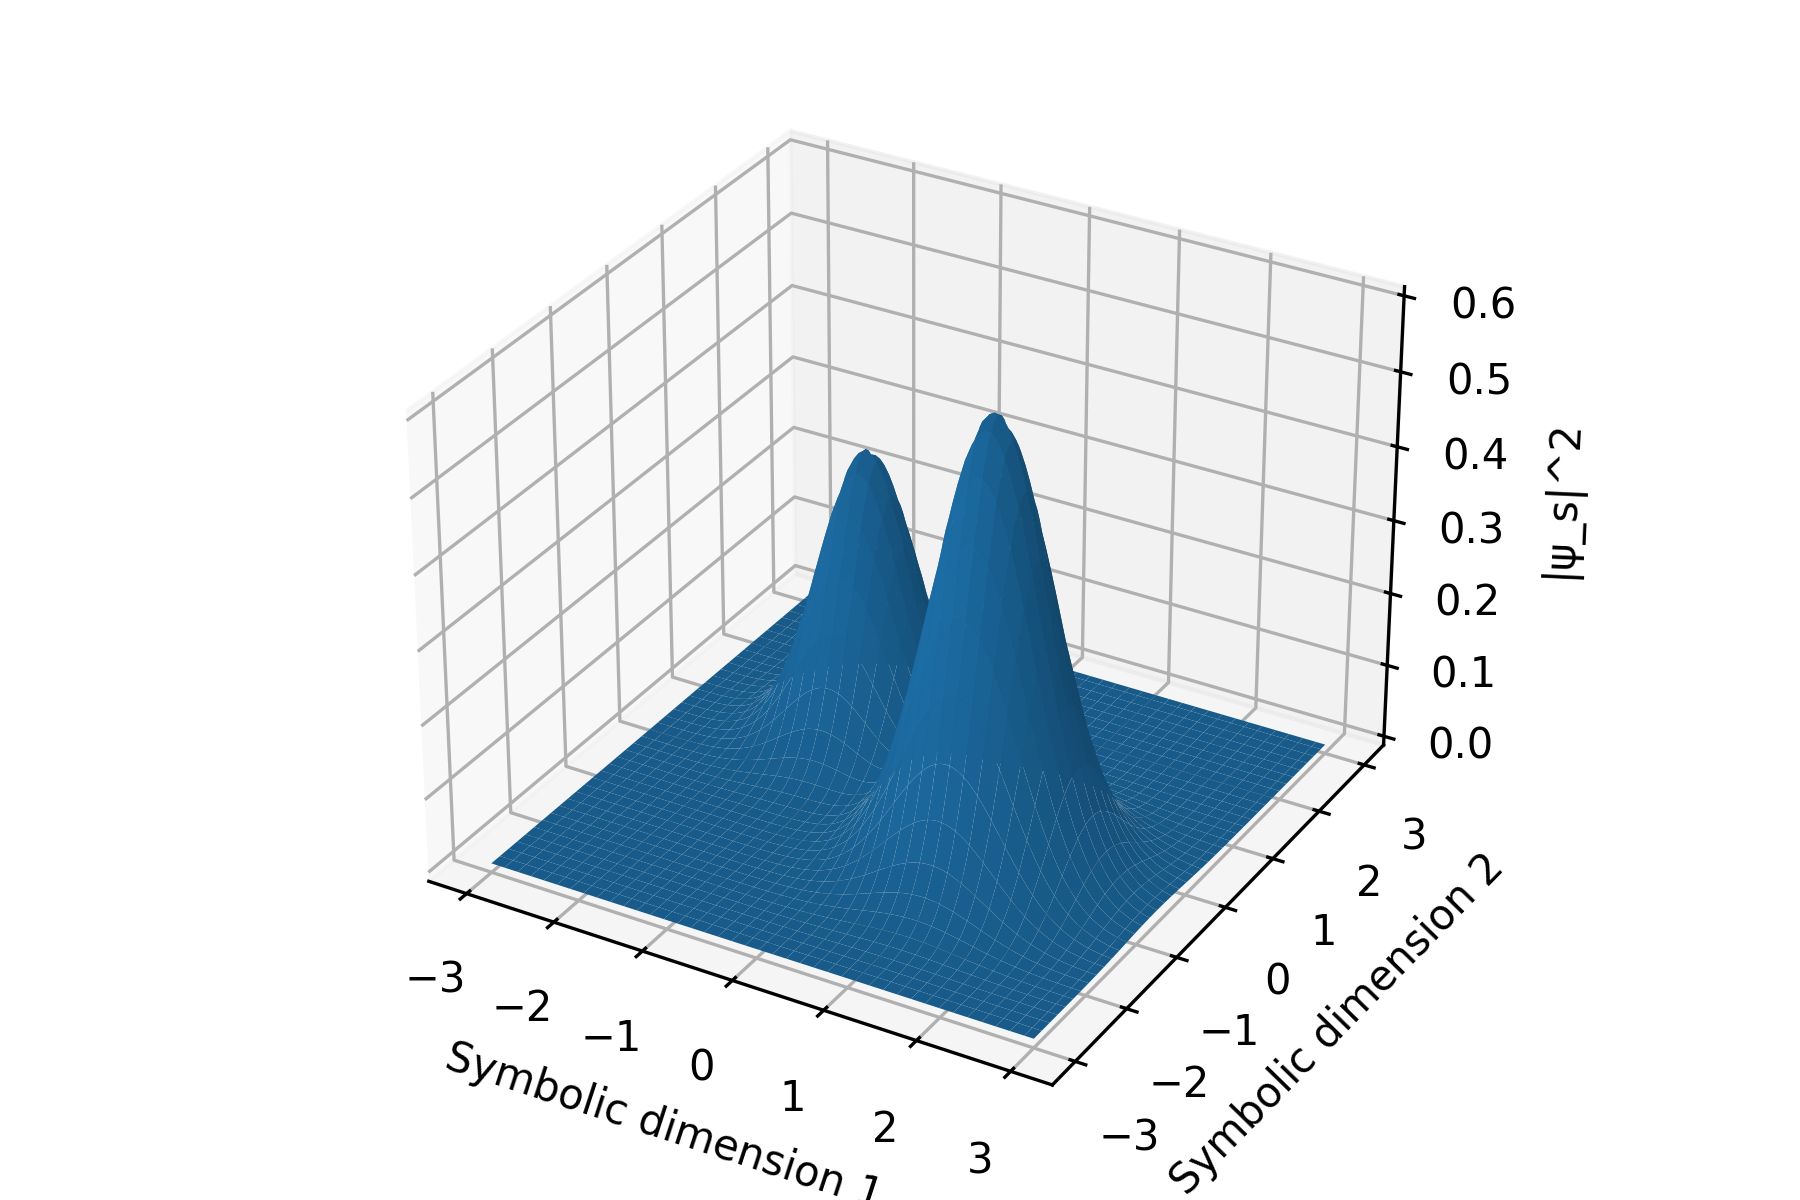
\includegraphics[width=.82\linewidth]{Fig1}
\caption{Symbolic wavefunction density \(|\psi_s|^2\) over a socio--symbolic space (3D surface; illustrative).}
\label{fig:wave3d}
\end{figure}

\begin{figure}[t]
\centering
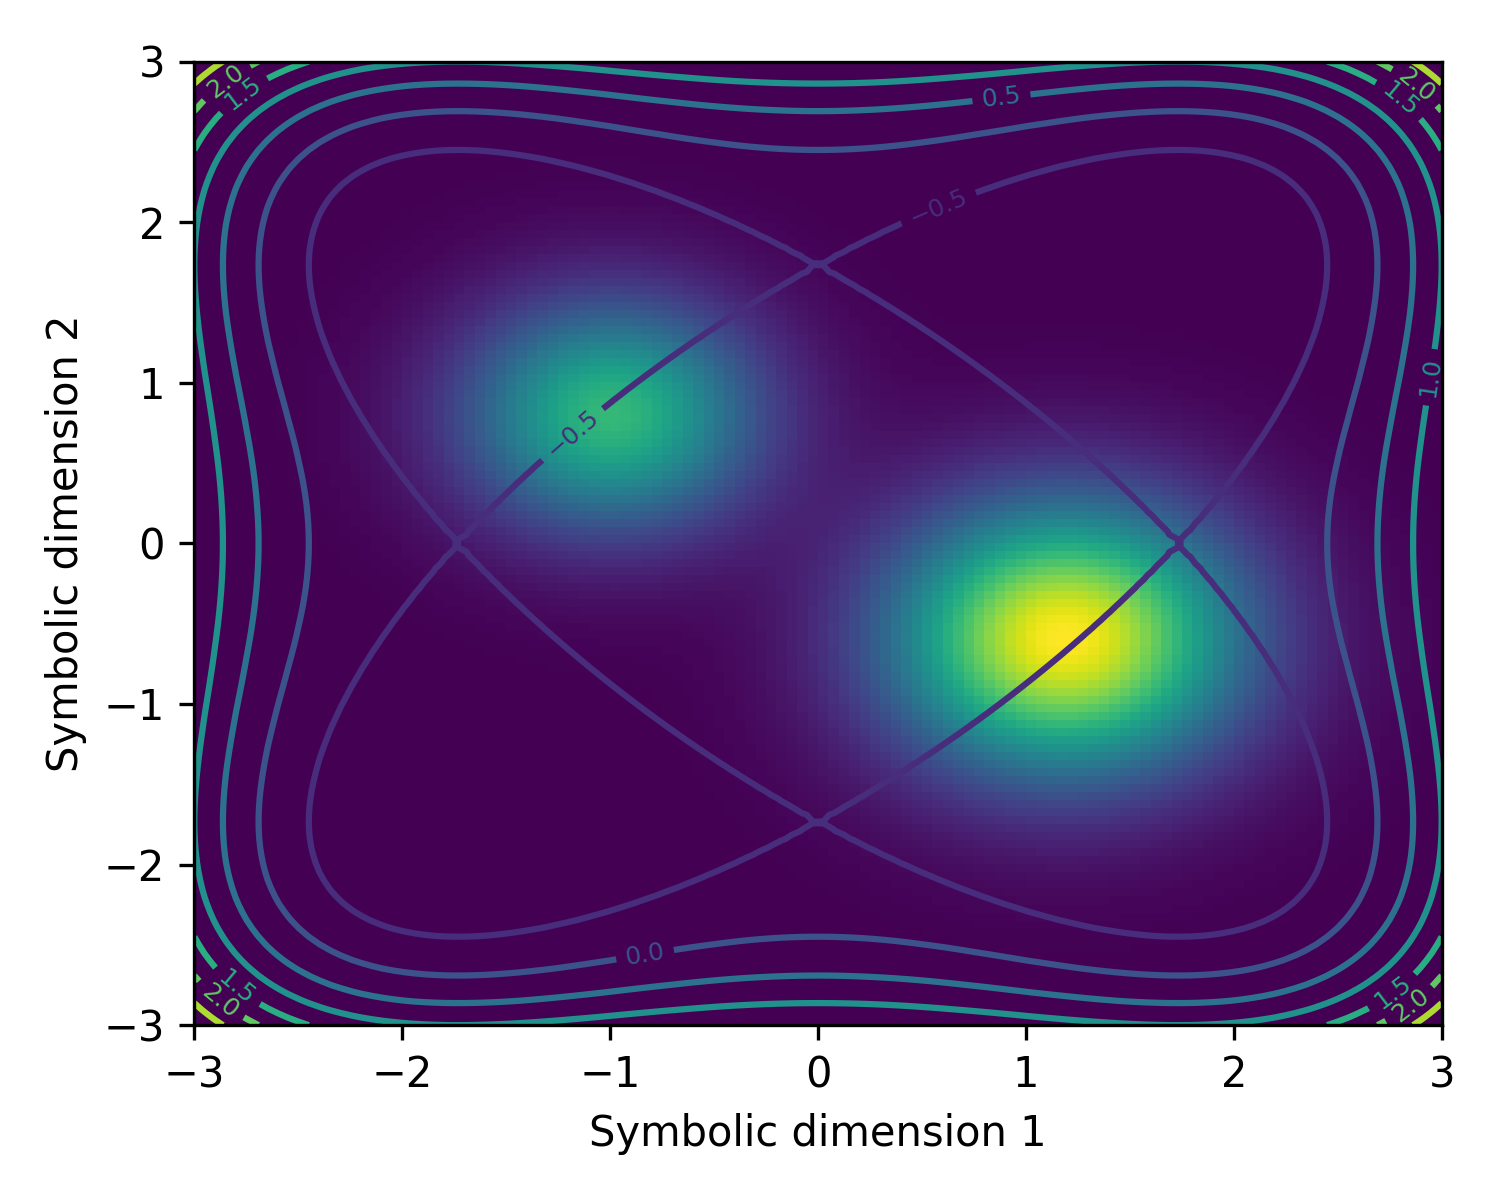
\includegraphics[width=.75\linewidth]{Fig2}
\caption{Density map \(|\psi_s|^2\) with normative potential contours \(V(x)\) (illustrative).}
\label{fig:densmap}
\end{figure}

\begin{figure}[t]
\centering
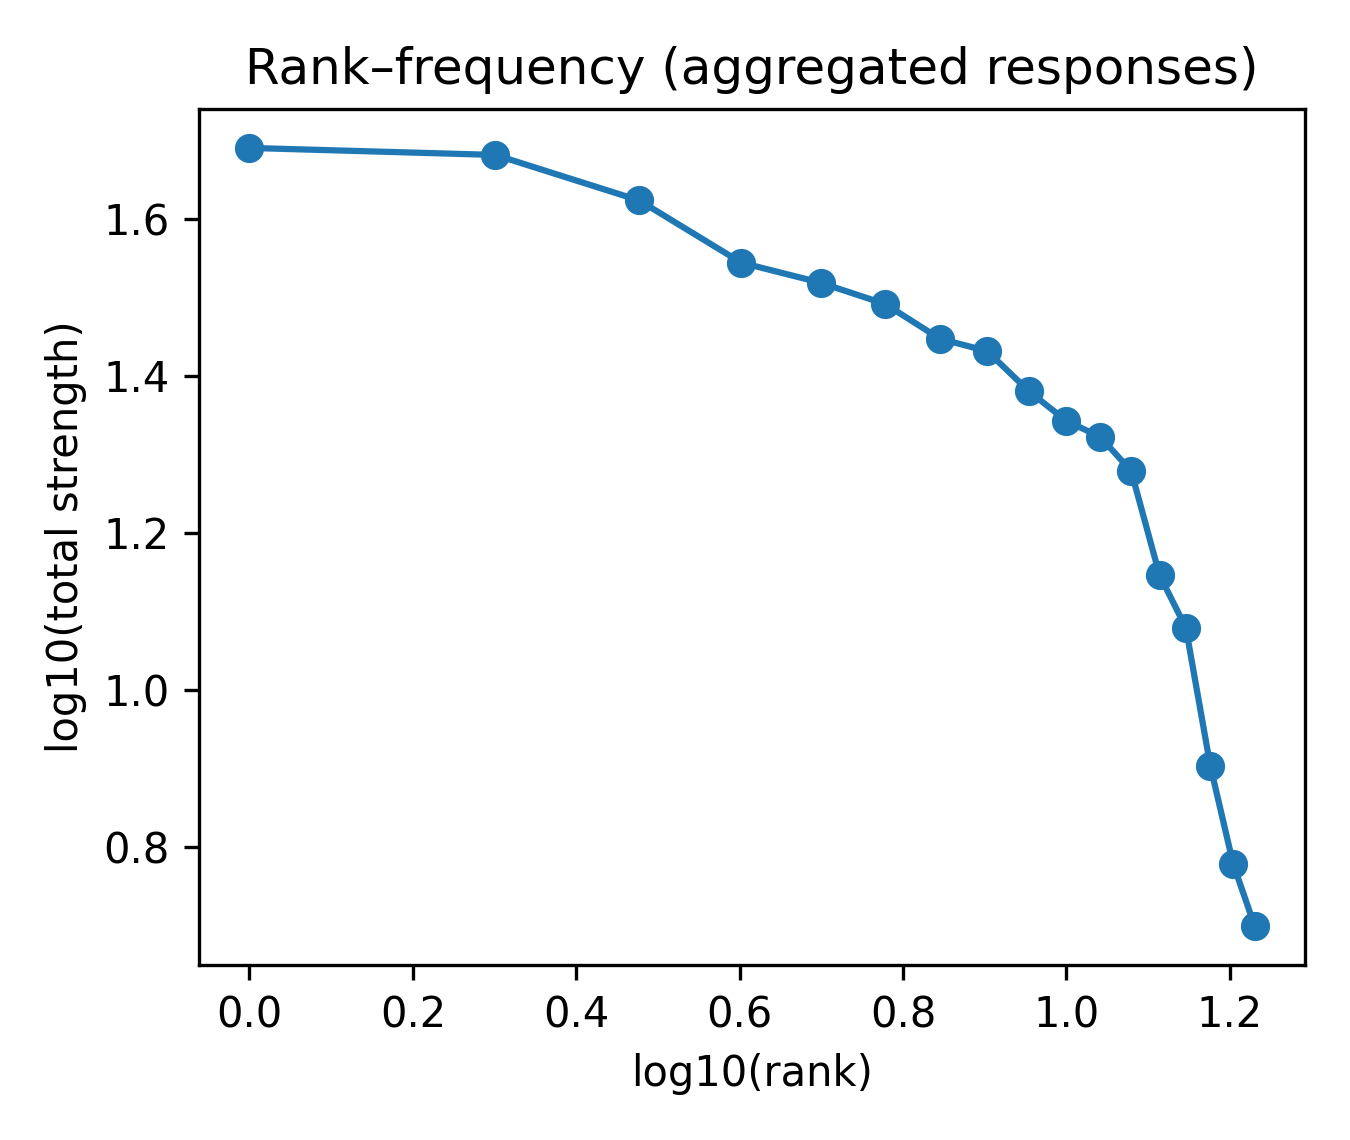
\includegraphics[width=.66\linewidth]{Fig3}
\caption{Rank--frequency (log--log) for aggregated responses (SWOW-style subset).}
\label{fig:rankfreq}
\end{figure}

\bmhead{Acknowledgments}
We thank collaborators for discussions on structural analogies and complex systems.

\bmhead{Author Contributions}
Conceptualization, formal analysis, writing---original draft: D.A.; writing---review \& editing: D.A.

\bmhead{Funding}
No specific funding was received for this work.

\bmhead{Data Availability}
Supplementary materials and figure-generation code are provided with the submission; SWOW data are subject to original licensing.

\bmhead{Competing Interests}
The author declares no competing interests.

\bibliographystyle{sn-chicago}
\bibliography{references}


\end{document}
